% Chapter Help

\chapter{Theoretical Background} % Main chapter title

\label{Chapter3} % For referencing the chapter elsewhere, use \ref{Chapter1} 
Having discussed the measurement conditions, a brief overview of the underlying theory of the CP measurement is going to be given.\\
The reason for the introduction of this mechanism was the result of an attempt to keep the gauge invariance of the SM, since an addition of a mass term to the wave equations of the force carriers results in a supplementary non-gauge invariant term. For this reason, in the early 60s Peter Higgs \parencite{Reference1}, François Englert and Robert Brout~\parencite{Reference2} have introduced a mechanism (which has since become known as the Brout-Englert-Higgs mechanism), based on the assumption of a gauge-invariant potential with ground states which are not invariant under such symmetry transformations. Therefore, the symmetry of such a system is spontaneously broken, leading to non-zero mass terms. Since these terms increase with the mass of the particle they couple to, it follows that with a special choice of the ground state, one can obtain the correct masses of the gauge bosons.\\
Having introduced the Higgs potential, the newly defined field (the Higgs field) must also have excited states producing a particle (the Higgs boson). In 2012, it has been announced by the ATLAS collaboration at CERN \parencite{Higgs2,Higgs1}, that a neutral boson with a mass of 126 GeV with a significance of 5.9$\sigma$ has been found, which later has been identified as the Higgs boson. Thus, for this discovery, both Peter W. Higgs and François Englert have been awarded the Nobel prize the next year.\\
However, some physical properties of this recently discovered particle are still unknown. One interesting property of the SM Higgs is its parity; as of 2018, a pure CP-odd state has been excluded and for its vector boson couplings \parencite{PDG_source}. Assuming a mixing angle between the CP-odd and CP-even states however, the precision of the parameters becomes fairly low \parencite{PDG}. Therefore, there is still ongoing research on the CP-even and CP-odd mixed states, which might help us -- in the long run -- to understand the matter-antimatter imbalance in the Universe.\\
\section{Higgs Production and Decays}
There are mainly four Higgs-production mechanisms at the LHC, which are pictured in Fig. \ref{fig:Higgs_productions}. In this thesis, production and decay mechanisms are also going to be called channels in the following.
\begin{comment}
	\begin{figure}[h]
		\centering
		\feynmandiagram [horizontal=a to b] {
			i1 -- [fermion] a -- [fermion] i2,
			a -- [photon,edge label=\gamma] b,
			f1 -- [fermion] b -- [fermion] f2,
		};
		\feynmandiagram [horizontal=a to b] {
			i1 [particle=\(\pi^{0}\)] -- [fermion] a -- [fermion] i2,
			a -- [dashed] b,
			f1 -- [fermion] b -- [fermion] f2,
		};
	\end{figure}\\
	\begin{figure}[h]
		\centering
		\feynmandiagram [horizontal=a to b] {
			i1 -- [fermion] a -- [fermion] i2,
			a -- [photon,edge label=\gamma] b,
			f1 -- [fermion] b -- [fermion] f2,
		};
		\feynmandiagram [horizontal=a to b] {
		i1 [particle=\(\pi^{0}\)] -- [fermion] a -- [fermion] i2,
		a -- [dashed] b,
		f1 -- [fermion] b -- [fermion] f2,
		};
		\caption{Feynman Diagrams}
		\label{fig:Higgs_productions}
	\end{figure}\\
\end{comment}
\begin{figure}[h]
	\centering
	\includegraphics[width=0.7\linewidth]{Figures/Higgs-production_PDG_Huge_p183}
	\caption{Feynman diagrams of the four main Higgs production channels at the LHC \parencite{PDG_source}}
	\label{fig:Higgs_productions}
\end{figure}\\
In the first and most common production mechanism -- the so-called gluon-gluon fusion or ggH -- two gluons fuse through a top-loop into a Higgs boson, since they do not couple to it directly as massless particles. The second most common channel is the vector boson fusion (VBF) where two quarks radiate off $Z$ or $W$ bosons, which then produce a Higgs particle. In the third case called Higgsstrahlung, a Higgs boson is radiated by a $W$ or $Z$ produced by a fusion of an quark-antiquark pair. In the fourth and least common channel, a pair of top (or bottom) quarks are also produced as ``by-products''. \\
As mentioned in the introduction Ch. \ref{Chapter1}, one has already measured the parity of the Higgs boson for its vector boson couplings, favouring a CP-even state and being in consistency with the SM prediction. Nevertheless, studying the ditau decay channel, a new term emerges in the Lagrangian of the system, which gives rise to a possible mixing between CP-odd and CP-even states. In Fig. \ref{fig:Higgs_decays}, several decay mechanisms with corresponding branching ratios (BR) and uncertainties are listed, among which the $b\overline{b}$ event is the most dominant. However, there are several limitations measuring the bottom quark polarisation. For this reason, the ditau channel is going to be favoured in this thesis.
\begin{figure}[h]
	\centering
	%\subfigure{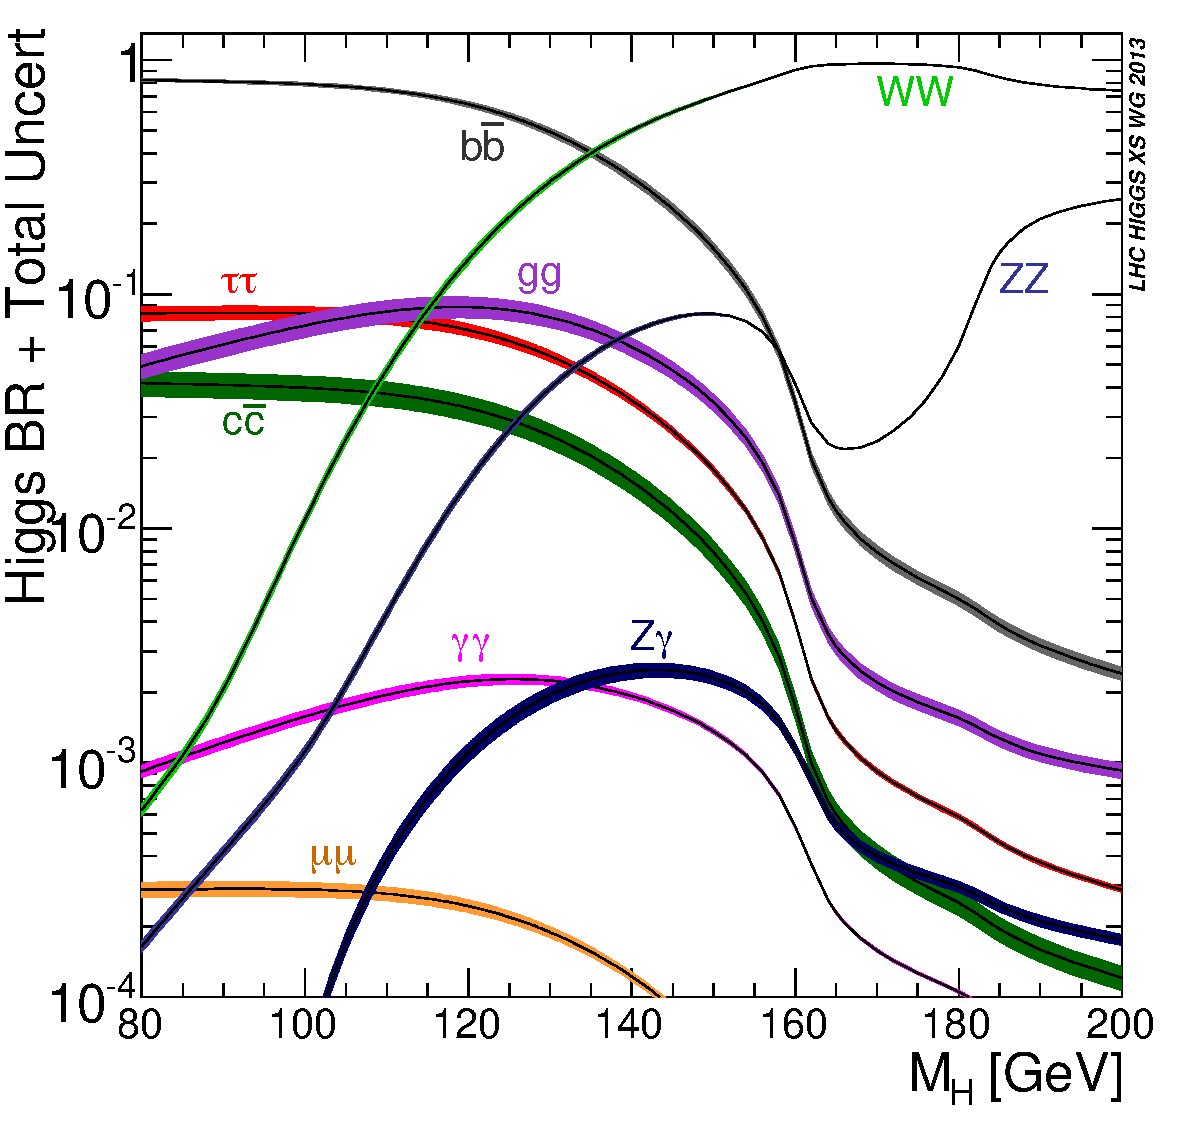
\includegraphics[width=0.4\linewidth]{Figures/Higgs_BR_LM_eps.pdf}}
	\subfigure{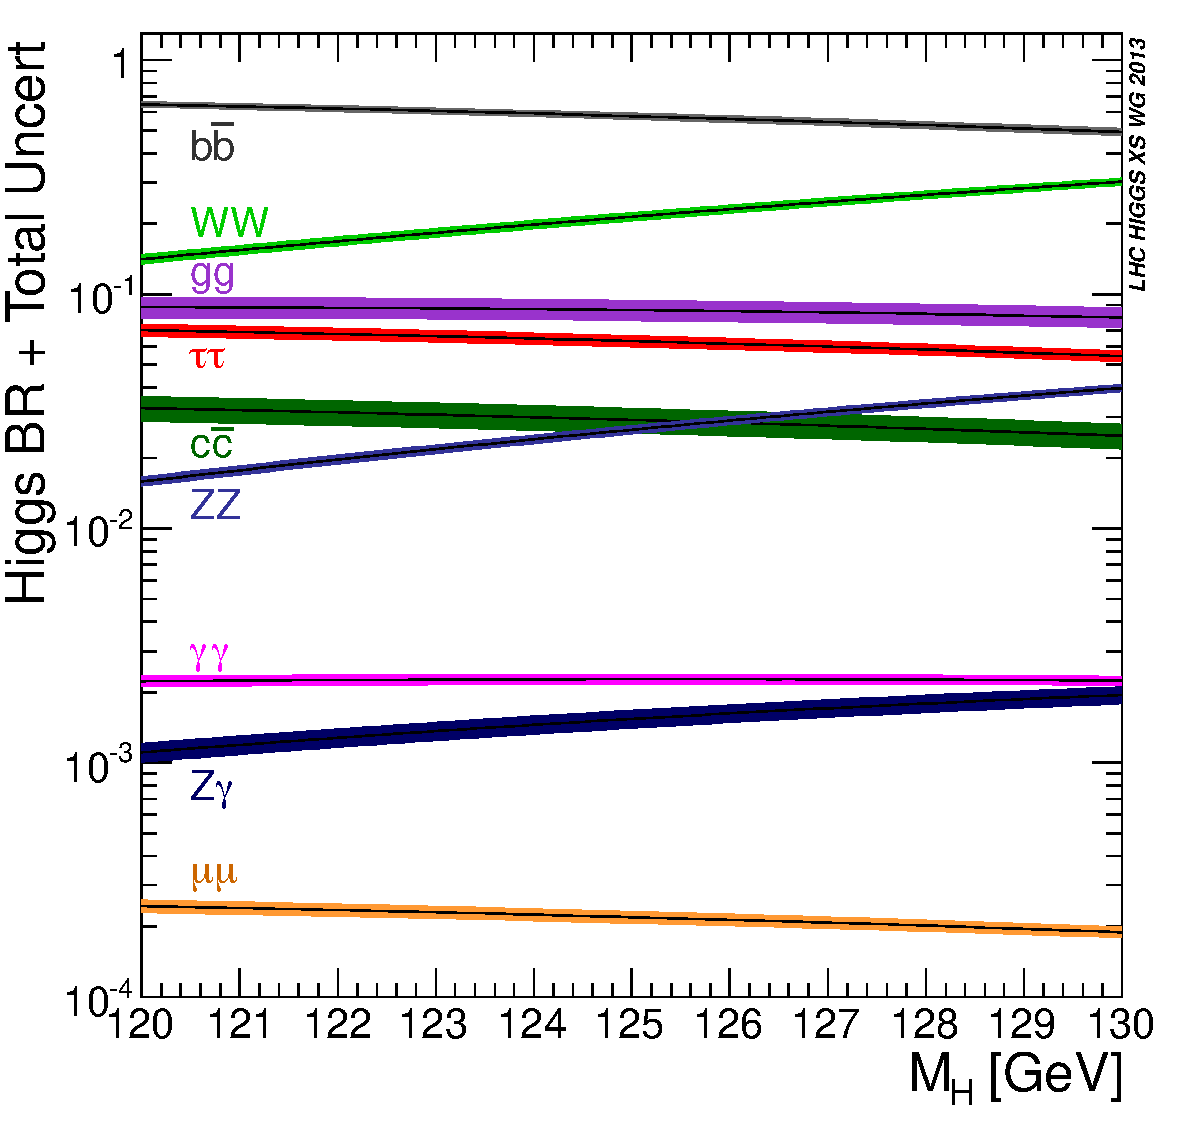
\includegraphics[width=0.6\linewidth]{Figures/Higgs_BR_120-130_eps.pdf}}
	\caption{The predicted branching ratios (BR) of Higgs boson decays as a function of the Higgs mass in the $m_H = 125$ GeV region \parencite{Higgs_decays}}
	\label{fig:Higgs_decays}
\end{figure}
\section{The CP-Mixing}
In order to proceed to the analysis of the decays, one should first introduce the charge conjugation operator $\hat{C}$ and the parity operator $\hat{P}$. \\
The parity operator is defined by the transformation $\hat{P}: \mathbb{R}^3 \rightarrow \mathbb{R}^3, \, \boldsymbol{x} \mapsto -\boldsymbol{x}$; i.e. it corresponds to a point reflection with respect to the origin. The charge conjugation operator $\hat{C}$ assigns to each particle its antiparticle, e.g. for a lepton $l$, $\hat{C}\ket{l} = \ket*{\overline{l}}$ holds. The combination of the two operators yields the $\hat{C}\hat{P}$-operator, which has two eigenvalues $\lambda_\pm=\pm 1$, where $\lambda_+=+1$ is called CP-even and $\lambda_-=-1$ is called CP-odd eigenstate. One can also show that a normalised superposition of a CP-even and a CP-odd eigenstate, $\ket{e}$ and $\ket{o}$, is not an eigenstate of the $\hat{C}\hat{P}$-operator anymore:
\begin{equation}
	\hat{C}\hat{P} \left(\cos\alpha\ket{e}+\sin\alpha\ket{o}\right) = \cos\alpha\ket{e}-\sin\alpha\ket{o} \neq \cos\alpha\ket{e}+\sin\alpha\ket{o}
\end{equation}
Now consider the Lagrangian $\mathcal{L}$ of the ditau decay channel \parencite{Berge_DY_bckg}, which is described by the Yukawa Langrangian $\mathcal{L}_Y$:
\begin{equation}
	\mathcal{L}_Y = -\left(\sqrt{2} G_F\right)^\frac{1}{2} m_\tau (a_\tau \overline{\tau}\tau+b_\tau \overline{\tau}i\gamma_5\tau)h
\end{equation}
where $G_F$ denotes the Fermi-constant and $a_\tau, b_\tau$ are the reduced dimensionless Yukawa coupling constants, $\gamma_5$ is the Dirac-matrix, and $\tau$ and $h$ are the Dirac and scalar fields respectively. Rewriting this Lagrangian as
\begin{center}
	\begin{tabular}{ll}
		$\mathcal{L}_Y $ & $= -\underbrace{\left(\sqrt{2} G_F\right)^\frac{1}{2} m_\tau\sqrt{a_\tau^2+b_\tau^2}}_\text{$g_\tau$} \left(\underbrace{\frac{a_\tau}{\sqrt{a_\tau^2+b_\tau^2}}}_\text{$\cos\varphi_\tau$} \overline{\tau}\tau+\underbrace{\frac{b_\tau}{\sqrt{a_\tau^2+b_\tau^2}}}_\text{$\sin\varphi_\tau$} \overline{\tau}i\gamma_5\tau\right)h$\\
		 & $= - g_\tau \left(\cos\varphi_\tau\overline{\tau}\tau+\sin\varphi_\tau\overline{\tau}i\gamma_5\tau\right)h$
	\end{tabular}
\end{center}
with an effective coupling strength $g_\tau$, one can see that $\varphi_\tau$ describes a degree of mixing between the scalar and the pseudoscalar coupling, corresponding to CP-even and CP-odd scenarios. For this reason, $\varphi_\tau$ is going to be denoted as the mixing angle between these two states, and is going to be an object of key importance in this thesis.\\
In case of the Higgs vector boson coupling discussed above the parity was found to be even. Current ATLAS and CMS measurements \parencite{CMS_CP_odd_exclusion,ATLAS_CP_odd_exclusion} disfavour a pure CP-odd scenario, i.e. where $\varphi_\tau = \frac{\pi}{2}$. The main constraint of this measurement is the indirect accessibility of $\varphi_\tau$, so one needs to find and measure an observable, which is related to it.
\section{The IP method}
\label{sec:IP_method}
There are multiple possible final states concerning the taus in the $H\rightarrow\tau\tau$ decay channels which have to be considered separately for this problem. In the following section, this thesis is going to focus on the one-prong ($\tau^\pm \rightarrow \rho^\pm \nu_\tau \rightarrow \pi^\pm\pi^0\nu_\tau$, $\tau^\pm \rightarrow \nu_\tau\pi^\pm$) and leptonic ($\tau^\pm \rightarrow \nu_\tau\overline{\nu}_\mu \mu^\pm$) decays, which can be used to construct an observable related to $\varphi_\tau$. Since neutrinos cannot be detected in the detector, they are going to be omitted from the decay reactions in the following.\\
It has been shown in \parencite{Berge_1prong, Berge_CP_Prospects} that the angle between the $\tau$ decay planes is such an observable. For this, one has to reconstruct these planes, for which depending on the decay channel two methods can be used. In case of a two-pion decay, the 3-momentum of the two pions with the secondary vertex span a plane, which can be used for the $\varphi_\tau$-study. In case of a leptonic or a one-pion decay, one could use the plane spanned by the impact parameter vector (which is defined by the minimum distance between the straight line given by the momentum of the child particle and the primary vertex PV) of the charged child and the direction of its momentum. In order to gain an overview, these cases are shown in Fig.~\ref{fig:claudiadecayplanes}.
\begin{figure}[h]
	\centering
	\includegraphics[width=0.9\linewidth]{Figures/Claudia_decay_planes}
	\caption{CP-relevant decay plane reconstruction in case of one-pion/leptonic (left) or two-pion (right) decays. Here, the impact parameter vector is denoted by $\vec{n}$ and momenta by $\vec{q}$; the vector to the secondary vertex (SV) of $\tau$ decay is called $\vec{k}$ \parencite{Claudia_thesis}}
	\label{fig:claudiadecayplanes}
\end{figure}\\
Concerning the angle between the decay planes $\varphi^*$ defined by the child particles of the taus, the following distribution can be found between $\varphi_{CP}^*$ and $\varphi_\tau$ (where the star denotes the zero momentum frame of the visible decay products):
\begin{equation}
	\label{eq:CP_Star_Distribution}
	\frac{d\sigma}{d\varphi_{CP}^*} \sim const - \cos(\varphi_{CP}^*-2\varphi_\tau).
\end{equation}
where $\varphi_{CP}^*$ is defined as
\begin{equation}
	\varphi_{CP}^* = \left\lbrace\begin{array}{cc}
	\varphi^*, \bigskip &\text{if } \mathcal{O_{CP}^*}\geq 0\\
	2\pi-\varphi^*, \bigskip &\text{if } \mathcal{O_{CP}^*}< 0
	\end{array}\right.
\end{equation}
with an $\mathcal{O_{CP}^*}$ given by
\begin{equation}
	\mathcal{O_{CP}^*} = \boldsymbol{\hat{p}^*}_- \cdot (\boldsymbol{\hat{d}}_-^*\times\boldsymbol{\hat{d}}_+^*).
\end{equation}
Here, $\boldsymbol{\hat{d}_\pm^*}$ are the normalised impact parameter vectors (IP) of the $\tau^\pm$ daughter particles in the ZMF, and $\boldsymbol{\hat{p}}_-^*$ is the normalised 3-momentum vector of the negatively charged daughter particle in the ZMF. For two 1-pion decays, these observables have been shown in Fig. \ref{fig:decayplanesphistar}.
\begin{figure}[h]
	\centering
	\includegraphics[width=0.4\linewidth]{Figures/decay_planes_phi_Star}
	\caption{The definition of $\varphi_{CP}^*$, with corresponding decay planes spanned by the 3-momentum and impact parameter vectors $\vec{n}$ \parencite{Berge_CP_Prospects}}
	\label{fig:decayplanesphistar}
\end{figure}
\begin{figure}[h]
	\centering
	\includegraphics[width=0.6\linewidth]{Figures/Phi_star_distribution}
	\caption{Theoretical $\varphi_{CP}^*$ distributions for CP-even, CP-odd and maximum mixing angle scenarios \parencite{Berge_CP_Prospects}}
	\label{fig:phistardistribution}
\end{figure}\\
To summarise: the angle between the decay planes is related to the mixing angle $\varphi_\tau$ through Eq. \ref{eq:CP_Star_Distribution}, such that the reconstruction of these is a good basis to measure it. For this, in cases of one-prong ($\pi^\pm\pi^0$) decays of the $\tau$, one can take the plane spanned by the pions; in cases of the leptonic ($\mu$) or 1-pion hadronic decay channels, one has to calculate the impact parameter of the child particles to obtain the relevant plane for this study. One expects therefore in accordance with Eq. \ref{eq:CP_Star_Distribution} trigonometrical distributions, as pictured in Fig. \ref{fig:phistardistribution} for some theoretical cases, where also the flat distribution of the background ($Z/\gamma \rightarrow \tau\tau$) events is displayed. Assuming a mixing angle $\varphi_{CP}^* \neq 0$, the Higgs boson is not an eigenstate of the $\hat{C}\hat{P}$ operator, meaning parity is not conserved during its decays.


